\chapter{Distributed Constraints}
\label{ch:dconstraints}

\hyphenation{no-good}

%  +(.75,1.75) node[gray,fill=gray,circle,draw,text width=.25cm,inner
%  sep=0cm] {}

\newcommand{\graphgrid}[1]{%
  \draw #1 -- +(1.5,0) 
  +(0,.5) -- +(1.5,.5)
  +(0,1) -- +(1.5,1)
  +(0,1.5) -- +(1.5,1.5)
  +(0,0) -- +(0,1.5)
  +(.5,0) -- +(.5,1.5)
  +(1,0) -- +(1,1.5)
  +(1.5,0) -- +(1.5,1.5)
  +(0,0) node[above left] {$x_3$}
  +(0,.5) node[above left] {$x_2$}
  +(0,1) node[above left] {$x_1$}
  +(.25,1.75) node {\medbullet}
  +(.75,1.75) node {\textcolor{gray}{\medbullet}}
  +(1.25,1.75) node {$\medcirc$};
}

\newcommand{\drawxat}[4]{%
  \draw (.5cm*#3+#1cm,.5cm*#4+#2cm) -- +(.5,.5)
  +(.5,0) -- +(0,.5);}

\newcommand{\drawxatred}[4]{%
  \draw[gray] (.5cm*#3+#1cm,.5cm*#4+#2cm) -- +(.5,.5)
  +(.5,0) -- +(0,.5);}

\newcommand{\tc}[1]{%
  \textcolor{#1}{\medbullet}}

Most multiagent systems are characterized by a set of autonomous
agents each with local information and ability to perform an action
when the set of actions of all must be coordinated so as to achieve a
desired global behavior. In all these cases you own all the agents in
question and can program them to do whatever you want. Thus, there is
no need to properly incentivise them as there would be in an open
system, which we study in later Chapters. However, there is still the
problem of coordination. Since each agent only has local information
it might be hard for it to decide what to do.

In this chapter we look at some algorithms for performing distributed
search in cooperative multiagent systems where each agent has some
local information and where the goal is to get all the agents to set
themselves to a state such that the set of states in the system is
optimal. For example, imagine a group of small sensors in a field.
Each sensor can communicate only with those that are near him and has
to decide which of its modalities to use (sense temperature, point
radar North, point radar South, etc.) so that the group of sensors
gets a complete view of the important events in the field. Or, imagine
a group of kids who have been told to stand in a circle, each one must
move find a spot to stand on but the position of that spot depends on
everyone else's location. In these examples the agents have local
information, can take any one of their available actions at any time,
but the utility of their actions depends on the actions of others. We
find that many multiagent problems can be reduced to a distributed
constraints problem. Thus, the algorithms we present in this chapter
have many different applications.


\section{Distributed Constraint Satisfaction}
\label{sec:dcs}

We start by formally describing the problem. In a \td{constraint
  satisfaction problem} (\idxi{\acro{csp}}{CSP}) we are given a set of
variables, each with its own domain along with a set of constraints.
The goal is to set every variable to a value from its domain such that
no constraints are violated. Formally,

\begin{definition}[Constraint Satisfaction Problem]
  Given a set of variables $x_1$, $x_2$,\ldots,$x_n$ with domains $D_1,
  D_2,\ldots,D_n$ and a set of boolean constraints $P$ of the form
  $p_k (x_{k1}, x_{k2}, \ldots , x_{kj}) \rightarrow \{0,1\}$, find
  assignments for all the variables such that no constraints are
  violated.
\end{definition}


\begin{SCfigure}
  \begin{minipage}{1.0\linewidth}
  \begin{center}
    \begin{tikzpicture}[style=dstyle]
      \tikzstyle{every node}=[draw,circle,text width=1em];
      \node (a) at (0,0) {};
      \node (b) at (0,2) {};
      \node (c) at (2,2) {};
      \node (d) at (2,0) {};
      \node (e) at (1,4) {};
      \node (f) at (4,1) {};
      \draw (a) -- (b) -- (c) -- (d) -- (a);
      \draw (b) -- (e) -- (c);
      \draw (c) -- (f) -- (d);
    \end{tikzpicture}
  \end{center}
  \end{minipage}
  \caption{Sample graph coloring problem. You must color each node
    either black, white, or gray so that no two nodes connected by an
    edge have the same color. Can you find a coloring?}
  \label{fig:graphcoloring}
\end{SCfigure}

The most widely studied instance of a constraint satisfaction problem
is the graph coloring problem, shown in
figure~\ref{fig:graphcoloring}.  In this problem we are given a graph
and a set of colors. The problem is to find out if there is a way to
color each node with one of the given colors such that no two nodes
that are connected by an edge have the same color.  We can easily map
the graph coloring problem to the formal definition of a \acro{csp} by
considering each node to be a variable, the domains to be the set of
colors, and each edge becomes a constraint between its two nodes that
is true only if their values are different.  Notice that, in graph
coloring constraints are only over two variables instead of over any
set of variables as we find in the general constraint satisfaction
problem.

The constraint satisfaction problem is NP-complete. As such, me use
search algorithms to find a solution and hope that the actual running
time will be less than the worst-case exponential time. In practice we
find that there are many special cases where we can solve the problem
really fast. For example, in the \td{n-queens problem} we are given an
$8 \times 8$ chess board with $8$ queens for which we must find places
on the board such that no queen can take another queen.  This problem
is a special case of the \acro{csp} but it is one for which there are
algorithms that can find a solution very quickly for large numbers of
queens as the problem is under constrained.

\begin{SCfigure}
  \begin{minipage}{1.0\linewidth}
  \begin{codebox}
    \Procname{$\proc{depth-first-search-csp}(i,g)$}
    \li \If $i > n$ 
    \li \Then \Return $g$
        \End
    \li \For $v \in D_i$ 
    \li \Do \If setting $x_i \gets v$ does not violate any constraint in
    $P$ given $g$ 
    \li     \Then $g' \gets \proc{depth-first-search-csp}(i+1 , g + \{x_i \gets v\})$ 
    \li           \If $g' \neq \emptyset$
    \li           \Then \Return $g'$
    \li           \End
             \End
         \End
    \li \Return $\emptyset$
  \end{codebox}
  \end{minipage}
  \caption{A centralized depth first search algorithm for the \acro{csp}.
    Variable $g$ holds the partial assignment of variable values. The
    algorithm is called with
    $\proc{depth-first-search-csp}(1,\emptyset)$.}
  \label{fig:dfs-csp}
\end{SCfigure}

A simple but effective method for solving the centralized constraint
satisfaction problem is with the use of a \td{depth first search}
algorithm, as shown in figure~\ref{fig:dfs-csp}. The algorithm simply
chooses an arbitrary ordering for the variables.\mc{A common
  modification is to improve the variables' ordering.} On each call it
tries to set the current variable $x_i$ to all its possible values to
see which ones do not violate any of the constraints in $P$ given the
partial variable assignment $g$. Whenever a value $v$ works, the
algorithm adds that assignment to $g$ and recursively tries to assign
the next variable in the list. This algorithm performs a complete
search and is thus guaranteed to find a solution if one exists. Depth
first search is also practical because it only requires an amount of
memory that is linear on the number of variables, that is, it has
$O(n)$ memory usage.  As we shall see later in this chapter, some of
the distributed algorithms try to parallelize this basic algorithm.

\medskip

In the \td{distributed constraint satisfaction} (\idxi{\acro{dcsp}}{DCSP})
problem we give each agent one variable. The agent is responsible for
setting the value of its own variable. The agents do not know the
values of any other variable but can communicate with other agents.
Formally, we define:

\begin{definition}[Distributed Constraint Satisfaction Problem] Give
  each agent one of the variables in a \acro{csp}. Agents are
  responsible for finding a value for their variable and can find out
  the values of the other agents' variables via communication
\end{definition}

Usually the agents are limited so that they can only communicate with
their neighbors---the agents with whom they share a constraint. Some
algorithms, however, allow agents to communicate with any other agent.
Also, most algorithms assume that the agents know about all the
constraints that involve their variable. 

The \acro{dcsp} is pervasive in multiagent research and many
real-world problems can be reduced to a \acro{dcsp}, or a variation
thereof. As such, many \acro{dcsp} algorithms have been developed,
each one with its own set of strengths and weaknesses. In the next
sections we examine some of the most popular algorithms.

\subsection{Filtering Algorithm}
\label{sec:filtering}

Picture yourself as one of the agents. You know your constraints, the
domain of your variable, and the domain of the variables of your
neighbors. You can use this information to determine if any of the
values from your variable's domain is impossible. That is, if there is
a value which violates some constraint no matter what value one of
your neighbors uses then that value will clearly not be part of the
solution so you can get rid of it. Similarly, all other agents might
do the same.

\begin{SCfigure}
  \begin{minipage}{1.0\linewidth}
    \begin{codebox}
      \Procname{$\proc{filtering}()$}
      \li \For $j \in \{\text{neighbors of }i\}$ \hspace{3em}\Comment $i$ is this agent.
      \li \Do  $\proc{revise}(x_i,x_j)$
          \End
    \end{codebox}
    \begin{codebox}
      \Procname{$\proc{handle-new-domain}(j,D')$}
      \li $D_j \gets D'$
      \li $\proc{revise}(x_i,x_j)$
    \end{codebox}
    \begin{codebox}
      \Procname{$\proc{revise}(x_i,x_j)$}
      \li $\id{old-domain} \gets D_i$
      \li \For $v_i \in D_i$ 
      \li \Do \If there is no $v_j \in D_j$ consistent with $v_i$
      \li     \Then $D_i \gets D_i - v_i$
              \End
          \End
      \li \If $\id{old-domain} \neq D_i$
      \li \Then $\forall_{k \in \{\text{neighbors of } i\}} k.\proc{handle-new-domain}(i,D_i)$
           \End
    \end{codebox}
  \end{minipage}
  \caption{The filtering algorithm. Each agent $i$ executes
    $\proc{filtering}()$.}
  \label{fig:filtering}
\end{SCfigure}

This idea is implemented by the \td{filtering algorithm}
\cite{waltz75} shown in figure~\ref{fig:filtering}. Every agent $i$
executes the \proc{filtering} procedure which leads it to do a
\proc{revise} with every one of its neighbors' variables $x_j$. If the
agent does succeed in eliminating one or more values from its domain
it then tells its neighbors its new domain.  When an agent receives
new domains from its neighbors it again executes \proc{revise} for
those neighbors. This process repeats itself until all agents finish
their computations and no more messages are sent.

The filtering algorithm is guaranteed to stop since there are only a
finite number of values in all the domains and the algorithm only
sends a message when a value is eliminated from a domain. Once it
stops, the filtering algorithm might have reduced the size of some
domains. Unfortunately, it might stop at a point where one or more of
the agents still has many values in its domain. Thus, it can stop
before a solution is found.

\begin{SCfigure}
  \begin{minipage}{1.0\linewidth}
  \begin{center}
    \begin{tikzpicture}[style=dstyle]
      \node[draw,circle] (x1) at (1,2) {$x_1$};
      \node[draw,circle] (x2) at (0,0) {$x_2$};
      \node[draw,circle] (x3) at (2,0) {$x_3$};
      \draw (x1) -- (x2) -- (x3) -- (x1);
      \graphgrid{(.25,2.5)}
      \graphgrid{(-1,-2.5)}
      \graphgrid{(1.5,-2.5)}
      \drawxat{.25}{2.5}{2}{2}
      \drawxat{.25}{2.5}{0}{0}
      \drawxat{.25}{2.5}{0}{1}
      \drawxat{.25}{2.5}{2}{0}

      \drawxat{-1}{-2.5}{2}{2}
      \drawxat{-1}{-2.5}{0}{0}
      \drawxat{-1}{-2.5}{0}{1}
      \drawxat{-1}{-2.5}{2}{0}

      \drawxat{1.5}{-2.5}{2}{2}
      \drawxat{1.5}{-2.5}{0}{0}
      \drawxat{1.5}{-2.5}{0}{1}
      \drawxat{1.5}{-2.5}{2}{0}

      \draw (2,3.25) node[right] {\textbf{1}: \proc{revise}($x_1, x_3$)};
      \drawxatred{.25}{2.5}{1}{2}
      \drawxatred{-1}{-2.5}{1}{2}
      \drawxatred{1.5}{-2.5}{1}{2}
      \draw (-.25,-3) node {\textbf{2}: \proc{revise}($x_2, x_3$)};
      \drawxatred{-1}{-2.5}{1}{1}
    \end{tikzpicture}
  \end{center}
  \end{minipage}
  \caption{Filtering example. The agents start out with some
    prohibited colors as indicated by the black crosses. On the first
    step $x_1$ does his \proc{revise} and eliminates the color gray
    from consideration. It then tells everyone else about this. Then
    $x_2$ does its revise and eliminates the color gray from its
    domain.}
  \label{fig:filterex}
\end{SCfigure}


Figure~\ref{fig:filterex} shows an example of the filtering algorithm
as applied to the graph coloring problem. In this problem the agents
have three possible colors but start out with already limited domains
as indicated by the black crosses. For example, agent $x_1$ can only
be either black or gray. At the first step $x_1$ executes
\proc{revise}($x_1, x_3$) and realizes that since $x_3$ must be gray
that it cannot be gray. As such, it eliminates gray from its domain
and tells all the other agents about this. The other agents
incorporate this knowledge. Then, agent $x_2$ does a
\proc{revise}($x_2,x_3$) and realizes that it also can't be gray and
thus eliminates gray from its domain. At this point $x_2$ knows the
final configuration. When it tells the other agents about its new
domain then all the agents will also know the final solution.

In this example the filtering algorithm found a specific solution.
Unfortunately, this is a rare occurrence. More often we find that the
filtering algorithm only slightly reduces the size of the domains. For
example, if we run the example from figure~\ref{fig:filterex} but
start with all possible colors in all domains then the filtering
algorithm will not be able to do anything. That is, none of the agents
are able to eliminate any color from their domain because many
colorings are possible.

\begin{SCfigure}
  \begin{minipage}{1.0\linewidth}
  \begin{center}
    \begin{tikzpicture}[style=dstyle]
      \node[draw,circle] (x1) at (1,2) {$x_1$};
      \draw (x1)
      +(-.25,.75) node {$\medbullet$}
      +(.25,.75) node {$\medcirc$};
      \node[draw,circle] (x2) at (0,0) {$x_2$};
      \draw (x2)
      +(-.25,-.75) node {$\medbullet$}
      +(.25,-.75) node {$\medcirc$};
      \node[draw,circle] (x3) at (2,0) {$x_3$};
      \draw (x3)
      +(-.25,-.75) node {$\medbullet$}
      +(.25,-.75) node {$\medcirc$};
      \draw (x1) -- (x2) -- (x3) -- (x1);
    \end{tikzpicture}
  \end{center}
  \end{minipage}
  \caption{Example of a problem that does not have a solution and
    the filtering algorithm cannot that fact.}
  \label{fig:nosolfilter}
\end{SCfigure}

The filtering algorithm might also fail to eliminate values from the
domains even when no coloring exists. That is, the filtering algorithm
cannot reliably detect problems that do not have a solution. This
problem can be illustrated with the example in
figure~\ref{fig:nosolfilter}. Here the nodes have to choose between
either white or black. We know that there is no possible way to color
these nodes without violating a constraint. However, the filtering
algorithm will get stuck at the first step in this example and will
not be able to reduce the size of the domains. Namely, each agent
considers that if he is black then the other two could be white and if
he is white then the other two could be black. As such, no agent
eliminates colors from its domain.

\subsection{Hyper-Resolution Based Consistency Algorithm}

The reason the filtering algorithm fails for this example is because
the \proc{revise} function considers only the agent's own value and
one other agent's value at a time. More generally, we need to consider
the agent's value against all possible combinations of the values of
two of its neighbors, of three of its neighbors, and so on all the way
to considering the values of all of its neighbors at the same time.

More formally, we say that if an agent can find a suitable value
regardless of the values of $k$ of its neighbors then it can be
consistent with anything they might do. If we can say this for all
agents then we have achieved \tdi{$k$-consistency}{k-consistency}.

\begin{definition}[$k$-consistency]
  Given any instantiation of any $k-1$ variables that satisfy all
  constraints it is possible to find an instantiation of any
  k$^{th}$ variable such that all $k$ variable values satisfy all
  constraints.
\end{definition}

If we can prove that problem is $j$-consistent for $j=2,3,\ldots$ up
to some number $k$ then we could say that the problem is strongly
$k$-consistent.

\begin{definition}[Strongly $k$-consistent]
  A problem is \emph{strongly $k$-consistent} if it is
  $j$-consistent for all $j \leq k$.
\end{definition}

We now face the problem of proving that a particular \acro{dcsp} is
strongly $k$-consistent. Notice that the filtering algorithm
guarantees $2$-consistency since it ensures that all agents can find a
value regardless of the value any one of their neighbors might set. We
need to extend this procedure to more than one neighbor. This can be
done using the \td{hyper-resolution rule}.

\begin{definition}[Hyper-Resolution Rule]
  \begin{gather*}
    \,\,A_1 \vee A_2 \vee \cdots \vee A_m \\
    \neg (A_1 \wedge A_{11} \wedge \cdots) \\
    \neg (A_2 \wedge A_{21} \wedge \cdots)\\
    :\\
    \frac{\neg (A_m \wedge A_{m1} \wedge \cdots)}{\neg (A_{11} \wedge \cdots \wedge A_{21} \wedge \cdots \wedge A_{m1} \wedge \cdots )}.
  \end{gather*}
\end{definition}

The hyper-resolution rule is a simple deduction rule from formal logic
whose form just so happens to correspond exactly to what we need. The
idea is that the agents' domains can be represented as an OR statement
like the first one in the rule. For example, if agent $x_1$ can be
either gray, black, or white then we write $x_1 = \text{gray} \vee x_1
= \text{black} \vee x_1=\text{white}$. The constraints are represented
as negations like the one in the second line of the hyperesolution
rule. For example, if there is a constraint that says that $x_1$ and
$x_2$ cannot both be white we would write that as $\neg (x_1 =
\text{white} \wedge x_2 = \text{white}$.  Once we have represented
both the domain and the constraints in this logical form then we can
use the hyper-resolution rule to generate new constraints which are
added to the agent's knowledge and communicated to the other agents.
Each one of these new constraints is called a \td{nogood}.

We can use the hyper-resolution rule to implement a distributed
constraint satisfaction algorithm that, unlike the filtering
algorithm, will detect all cases where there is no solution and will
find a solution when there is one. The algorithm is basically the same
as the filtering algorithm but we modify the \proc{revise} function to
instead use the hyper-resolution to generate new nogoods. These
nogoods are then sent to the other agents. When an agent receives
nogoods from other agents it adds them to its set of nogoods. The
process continues until no new nogoods can be derived by any agent or
until a contradiction is reached. When a contradiction is found it
means that no solution exists to this problem.

We now show how the hyper-resolution algorithm would solve the problem
from figure~\ref{fig:nosolfilter}. Table~\ref{tab:hyperex} shows a few
of the initial statements in the agents' databases. Note that many of
the nogoods are missing due to space limitations but you can easily
infer them as they correspond to the constraints in the problem. One
possible run of the algorithm is as follows:

\begin{SCtable}
  \begin{minipage}{1.0\linewidth}
  \begin{center}
    \begin{tabular}{rccc}\toprule
       & $\mathbf{x_1}$ & $\mathbf{x_2}$ & $\mathbf{x_3}$ \\ \cmidrule{2-4}
       & \phantom{$\neg ($}$x_1 = \medcirc \vee x_1 = \medbullet$\phantom{$)$} &
      \phantom{$\neg ($}$x_2 = \medcirc \vee x_2 = \medbullet$\phantom{$)$} &
      \phantom{$\neg ($}$x_3 = \medcirc \vee x_3 = \medbullet$\phantom{$)$}  \\ 
       & $\neg (x_1 = \medcirc \wedge x_2 = \medcirc)$ &
      $\neg (x_1 = \medcirc \wedge x_2 = \medcirc)$ &
      $\neg (x_1 = \medcirc \wedge x_2 = \medcirc)$   \\ 
      Time & $\neg (x_1 = \medbullet \wedge x_2 = \medbullet)$ &
      $\neg (x_1 = \medbullet \wedge x_2 = \medbullet)$ &
      $\neg (x_1 = \medbullet \wedge x_2 = \medbullet)$ \\ \midrule
      1 & \textcolor{black}{$\neg(x_2 = \medcirc \wedge x_3 = \medbullet)$} & 
      \textcolor{black}{$\neg(x_2 = \medcirc \wedge x_3 = \medbullet)$} & 
      \textcolor{black}{$\neg(x_2 = \medcirc \wedge x_3 =
        \medbullet)$}\\ 
      2 & \textcolor{black}{$\neg(x_2 = \medbullet \wedge x_3 = \medcirc)$} &
      \textcolor{black}{$\neg(x_3 = \medbullet)$}&
      \textcolor{black}{$\neg(x_2 = \medbullet \wedge x_3 = \medcirc)$}  \\ 
      3 & &
      \textcolor{black}{$\neg(x_2 = \medbullet \wedge x_3 = \medcirc)$}&  
      \textcolor{black}{$\neg(x_3 = \medcirc)$} \\ 
      4 & &
      \textcolor{black}{$\neg(x_3 = \medcirc)$}  &  
      \textcolor{black}{$\neg(x_3 = \medbullet)$} \\ \bottomrule
    \end{tabular}
  \end{center}
  \end{minipage}
  \caption{Example databases for a sample run of the hyper-resolution
    based consistency algorithm as applied to the graph of
    figure~\ref{fig:nosolfilter}. Only a few of the nogoods produced
    by the graph's constraints are shown due to space constraints. You
    can infer the rest. New statements are added starting at time 1.}
  \label{tab:hyperex}
\end{SCtable}
% \only<presentation>{
%   \begin{center}
%     \begin{tikzpicture}[line width=1pt]
%       \node[draw,circle] (x1) at (1,1.5) {$x_1$};
%       \draw (x1)
%       +(-.25,.75) node {$\medbullet$}
%       +(.25,.75) node {$\medcirc$};
%       \node[draw,circle] (x2) at (0,0) {$x_2$};
%       \draw (x2)
%       +(-.25,-.75) node {$\medbullet$}
%       +(.25,-.75) node {$\medcirc$};
%       \node[draw,circle] (x3) at (2,0) {$x_3$};
%       \draw (x3)
%       +(-.25,-.75) node {$\medbullet$}
%       +(.25,-.75) node {$\medcirc$};
%       \draw (x1) -- (x2) -- (x3) -- (x1);
%     \end{tikzpicture}
%   \end{center}}
Let $x_1$ start out by doing
\begin{center}
\begin{tabular}{c}
  \phantom{$\neg ($}$x_1 = \medcirc \vee x_1 = \medbullet$\phantom{$)$} \\
  $\neg(x_1 = \medcirc \wedge x_2 = \medcirc)$ \\
  $\neg(x_1 = \medbullet \wedge x_3 = \medbullet)$ \\ \midrule
  $\neg(x_2 = \medcirc \wedge x_3 = \medbullet)$
\end{tabular}
\end{center}
at time 1. It then sends $\neg(x_2 = \medcirc \wedge x_3 =
\medbullet)$ to $x_2$ and $x_3$. $x_2$ then can do

\begin{center}
  \begin{tabular}{c}
    \phantom{$\neg ($}$x_2 = \medcirc \vee x_2 = \medbullet$\phantom{$)$} \\
    $\neg(x_2 = \medcirc \wedge x_3 = \medbullet)$ \\
    $\neg(x_2 = \medbullet \wedge x_3 = \medbullet)$ \\ \midrule
    $\neg(x_3 = \medbullet)$
  \end{tabular}
\end{center}
Meanwhile, $x_1$ can do
\begin{center}
  \begin{tabular}{c}
    \phantom{$\neg ($}$x_1 = \medcirc \vee x_1 = \medbullet$\phantom{$)$} \\
    $\neg(x_1 = \medbullet \wedge x_2 = \medbullet)$ \\
    $\neg(x_1 = \medcirc \wedge x_3 = \medcirc)$ \\ \midrule
    $\neg(x_2 = \medbullet \wedge x_3 = \medcirc)$ 
  \end{tabular}
\end{center}
$x_1$ then sends the nogood $\neg(x_2 = \medbullet \wedge x_3 = \medcirc)$ to
$x_2$ and $x_3$. Using this message, $x_2$ can now do
\begin{center}
  \begin{tabular}{c}
    \phantom{$\neg ($}$x_2 = \medcirc \vee x_2 = \medbullet$\phantom{$)$} \\
    $\neg(x_2 = \medcirc \wedge x_3 = \medcirc)$ \\
    $\neg(x_2 = \medbullet \wedge x_3 = \medcirc)$ \\ \midrule
    $\neg(x_3 = \medcirc)$
  \end{tabular}
\end{center}
$x_2$ then sends $\neg(x_3 = \medcirc)$ and $\neg(x_3 = \medbullet)$
to $x_3$. Using this message, $x_3$ can then do
\begin{center}
  \begin{tabular}{c}
    $x_3 = \medcirc \vee x_3 = \medbullet$ \\
    $\neg(x_3 = \medcirc)$ \\
    $\neg(x_3 = \medbullet)$ \\ \midrule
    Contradiction
  \end{tabular}
\end{center}
This last step derives a contradiction which means that the algorithm
has been able to prove that no solution exists.

In practice, the hyper-resolution algorithm is very slow because there
is often little guidance as to which nogoods should be derived first.
That is, at any one time each agent can derive a large number of
different nogoods. Most of these are useless to the other agents and
there is no easy way for the agent to determine which nogoods might be
most useful since that would require that it also know about the other
agents' databases. As such, we find that in practice the
hyper-resolution algorithm spends a lot of time deriving useless
nogoods. This is especially true as the size of the nogoods---their
number of terms---increases. Also, if the problem does have a solution
then the algorithm only stops when all the agents prove to themselves
that they cannot generate any new nogood, which can take a very long
time. In summary, hyper-resolution in its raw form is impractical for
most cases with the possible exception of highly over-constrained
problems.

\subsection{Asynchronous Backtracking}

Earlier, in figure~\ref{fig:dfs-csp}, we saw a depth first search
algorithm for solving a constraint satisfaction problem. The algorithm
sets a variable to a specific value and, recursively, tries to set a
new variable to some value which would not violate any of the
constraints with existing values. If no such value exists the
algorithm backs up and re-sets one of the variables it has already
set. This type of depth first search is also known as a
\td{backtracking} algorithm because we set the variables to some
values and then if there is a conflict we backtrack, unset
variables, and try again with different values.

The \td{asynchronous backtracking} algorithm (\idxi{\acro{abt}}{ABT}),
is a distributed asynchronous version of the centralized depth first
search algorithm for constraint satisfaction \cite{yokoo00a}.
\acro{abt} performs the same kind of search but it does so via the use
of messages between agents and under the understanding that only the
owner of the variable can change its value.

The \acro{abt} algorithm also implements some performance improvements
on the basic depth first search. As we mentioned earlier, there is
often much to be gained by properly ordering the variables.  In
general, we want to place variables that are involved in more
constraints towards the top of the tree and search them first so as to
avoid having to do some backtracking later on. This heuristic has been
shown to work well and is employed by \acro{abt}.

Each agent $i$ in \acro{abt} is responsible for variable $x_i$.  All
agents are given a fixed \id{priority} ordering, from 1 to $n$.  Each
agent $i$ can change the value of its variable $x_i$. The agents keep
track of the others' variables in \id{local-view}. The list of
\id{neighbors} is initially set to be just the other agents with whom
the agent shares a constraint but, as we will see, this list can grow.
The agents find out other agents' variable values by sending messages.
There are only three types of messages that \acro{abt} sends. Thus,
only three remote procedures need to be implemented.

\begin{enumerate}
\item $\proc{handle-ok?}(j, x_{j})$ where $j$ is the name of another agent
  and $x_j$ is its current variable value. This message asks the
  receiver if that assignment does not violate any of his constraints.

\item $\proc{handle-nogood}(j, \id{nogood})$ which means that $j$ is
  reporting that it can't find a value for his variable because of
  $nogood$.

\item $\proc{handle-add-neighbor}(j)$ which requests the agent to add
  some other agent $j$ as its neighbor. This message is handled by simply
  adding that agent to \id{neighbors}.
\end{enumerate}

\begin{SCfigure}
  \begin{minipage}{1.0\linewidth}
  \begin{codebox}
    \Procname{$\proc{handle-ok?}(j, x_{j})$}  
    \li $\id{local-view} \gets \id{local-view} + (j, x_j)$
    \li $\proc{check-local-view}()$
  \end{codebox}

  \begin{codebox}
    \Procname{$\proc{check-local-view}()$}
    \li \If $\id{local-view}$ and $x_i$ are not consistent
    \li \Then \If no value in $D_i$ is consistent with $\id{local-view}$
    \li       \Then $\proc{backtrack}()$
    \li       \Else select $d \in D_{i}$ consistent with $\id{local-view}$
    \li       $x_i \gets d$
    \li       $\forall_{k \in \id{neighbors}} \;k.\proc{handle-ok?}(i,x_i)$
              \End
       \End
  \end{codebox}
  \begin{codebox}
    \Procname{$\proc{handle-add-neighbor}(j)$}
    \li $\id{neighbors} \gets \id{neighbors} + j$
  \end{codebox}

  \begin{codebox}
    \Procname{$\proc{handle-nogood}(j, \id{nogood})$}  
    \li record $nogood$ as a new constraint
    \li \For $(k,x_k) \in \id{nogood}$ where $k \notin \id{neighbors}$
    \li \Do $k.\proc{handle-add-neighbor}(i)$
    \li $\id{neighbors} \gets \id{neighbors} + k$
    \li $\id{local-view} \gets \id{local-view} + (k,x_k)$
    \End
    \li $\id {old-value} \gets x_i$
    \li $\proc{check-local-view}()$
    \li \If $\id{old-value} \neq x_i$
    \li \Then $j.\proc{handle-ok?}(i,x_i)$
    \End
  \end{codebox}

  \begin{codebox}
    \Procname{$\proc{backtrack}()$}
    \li $nogoods \gets \left\{V\,|\,V=\right.$ inconsistent subset of
    \id{local-view} using hyper-resolution rule$\}$
    \li \If an empty set is an element of $nogoods$
    \li \Then broadcast that there is no solution
    \li       terminate this algorithm
    \End
    \li \For $V \in nogoods$
    \li    \Do select $(j, x_j)$ where $j$ has lowest priority in $V$
    \li        $j.\proc{handle-nogood}(i,V)$
    \li        $\id{local-view} \gets \id{local-view} - (j, x_j)$
    \End
    \li $\proc{check-local-view}()$
  \end{codebox}
  \end{minipage}
  \caption{\acro{abt} algorithm. All agents start by setting
    themselves to some color and invoking a \proc{handle-ok?} on all
    their neighbors. After this they become event driven.}
  \label{fig:abt}
\end{SCfigure}

The full algorithm can be seen in figure~\ref{fig:abt}. All agents
start out by setting their $x_i$ variable to some value and then
asking all their neighbors to \proc{handle-ok?} After that they become
event-driven, handling messages as they arrive. \acro{abt} assumes
that messages are never lost and arrive and in the same order they
were sent.

\begin{SCfigure}
  \begin{minipage}{1.0\linewidth}
  \begin{center}
    \begin{tikzpicture}[style=dstyle]
      \node[draw,circle] (x1) at (2,4) {$x_1$};
      \draw (x1)
      +(-.25,.75) node {$\medbullet$}
      +(.25,.75) node {$\medcirc$};
      \node[draw,circle] (x2) at (0,0) {$x_2$};
      \draw (x2)
      +(-.25,-.75) node {$\medbullet$}
      +(.25,-.75) node {$\medcirc$};
      \node[draw,circle] (x3) at (4,0) {$\mathbf{x_3}$};
      \draw (x3)
      +(-.25,-.75) node {$\medbullet$};
      \draw (x1) -- (x2)
      (x3) -- (x1);


      \draw (0,0) node[circle,fill=white] {$x_2$};
      \draw (4,0) node[circle,fill=black] {\textcolor{white}{$x_3$}};

      \draw[-angle 90,gray] (x2) .. controls +(0,.5) and +(-.5,-.5) .. 
      node[black,above,sloped] {\textbf{1:} $: \mathbf{ok?} (x_2, \medcirc)$}
      (x1);
      \draw[-angle 90,gray] (x3) .. controls +(0,.5) and +(.5,-.5) .. 
      node[black,above,sloped] {\textbf{1:} $ \mathbf{ok?} (x_3, \medbullet)$} (x1);
      
      \draw (3,4.5) node[black,right] 
      {\textbf{2:} $\id{local-view} = (x_2,\medcirc), (x_3, \medbullet)$};


      \draw[-angle 90,gray] (x1) .. controls +(2,-.5) and +(1,.5) .. 
      node[black,above,sloped] {\textbf{3:} $\mathbf{nogood} (x_2 = \medcirc \wedge
        x_3 = \medbullet)$} (x3);

      \draw[gray] (x3) -- node[black,above] {\textbf{4:} Added link} (x2);

      \draw[-angle 90,gray] (x2)
      .. controls +(.5,.6) and +(-.5,.6) .. 
      node[above,sloped,black] {\textbf{5:} $\mathbf{ok?} (x_2, \medcirc)$}
      (x3);

      \draw (4.3,-.3) node[right,black] 
      {\textbf{5:} $\id{local-view} = (x_2,\medcirc)$};

      \draw[-angle 90,gray] (x3)
      .. controls +(-.5,-.5) and +(.5,-.5) .. 
      node[below,sloped,black] {\textbf{6:} $\mathbf{nogood} (x_2, \medcirc)$}
      (x2);

    \end{tikzpicture}
  \end{center}
  \end{minipage}
  \caption{\acro{abt} example. The numbers preceding each message indicate
    the time at which the particular action took place. Only the first
    six steps are shown.}
    \label{fig:abtex}
\end{SCfigure}

The procedure \proc{check-local-view} checks that the agent's current
value $x_i$ is consistent with the values it thinks its neighbors
have. If not then it checks to see if it can find some other value
that will work. If it can't find one then this means it must
\proc{backtrack} and find a new value. If it can then it sets $x_i$ to
that value and informs its neighbors.

Nogoods are handled by \proc{handle-nogood}. The first thing this
procedure does is to see if any of the agents in the nogood is not in
\id{neighbors} so it can add it. This step is needed to ensure the
algorithm will arrive at a correct answer. The nogood is added to the
set of constraints and \proc{check-local-view} is called to ensure
there are no conflicts.

Finally, the \proc{backtrack} procedure is responsible for generating
and sending new nogoods. As we saw, it is only called when there is no
way for the agent to set is value so that no constraints are violated.
This means that someone else must change their value. That someone
else is the agent with the lowest priority in the nogood.
\proc{backtrack} first uses the hyper-resolution rule (or similar) to
generate one or more nogoods.\mc{Some versions of \acro{abt} use one
  nogood in line~1 of \proc{backtrack}, others use more.} Each one of
these nogoods is then sent to the agent in that nogood that has the
lowest priority. Also, if the hyper-resolution generated a
contradiction, represented as an empty set then this means that no
solution exists and thus the algorithm is terminated.

Notice that, since the nogoods are always sent to the lowest priority
agent and the agents have linear priorities, the nogoods always flow
from the high priority agents to the low priority agents. Namely, the
highest priority agent will never receive a nogood, the second highest
priority agent will only receive nogoods from the highest priority
agent, and so on.  This suggests to us that the lower priority agents
will end up doing more work.

\netlogo{ABTgc} An example of \acro{abt} at work can be seen in
figure~\ref{fig:abtex}. Here agents $x_2$ and $x_3$ start by setting
their colors to be gray and black, respectively, and asking $x_1$ to
\proc{handle-ok?}. Agent $x_1$ then generates a new nogood and sends a
\id{nogood} to $x_3$. $x_3$ notices that $x_2$ is in the nogood but
not in his \id{neighbors} and so adds it as his neighbor and asks
$x_2$ to add him as a neighbor. In response to this $x_2$ asks $x_3$
to \proc{handle-ok?} with his new color. Agent $x_3$ uses $x_2$'s new
color to generate a new nogood that it sends to $x_2$. The figure ends
at this point but the algorithm would continue with $x_2$ realizing
that it must set itself to black and sending the appropriate
\proc{handle-ok?} messages, and so on.

The \acro{abt} algorithm has been shown to be complete.

\begin{theorem}[\acro{abt} is Complete]
  The \acro{abt} algorithm always finds a solution if one exists and
  terminates with the appropriate message if there is no solution
  \cite{yokoo98a}.
\end{theorem}
\begin{proof}
  The proof works by induction. In order to prove it we must first
  show that the agent with the highest priority never enters an
  infinite loop. Then show that given that all the agents with lower
  priority that $k$ never fall into an infinite loop then $k$ will not
  fall into an infinite loop.
\end{proof}

Unfortunately, after running a few examples of this algorithm one
quickly notices some problems. The most important is the uneven
division of labor. In \acro{abt} the lowest priority agent ends up
doing many times more work than the highest priority agents, which is
reflected by the number of messages each agent receives. The
difference only gets worse as the number of agents increases. Another
drawback is the fact that in practice \acro{abt} can take very long as
it also suffers from the same problem as regular backtracking. That
is, if the high priority agents make bad decisions (choose colors that
will not work) then it takes a long time to fix these as all the other
agents have to prove that those colors will not work by trying all
possible combinations of their colors. In the graph coloring problem
we notice that the time to solve a problem increases exponentially as
the ratio of edges to nodes increases. This means that as the problem
becomes more constrained the time to find a solution explodes.

\netlogo{ABTmm}Another possible improvement to \acro{abt} can be found
in line~1 of \proc{backtracking} which tells us to find new nogoods.
As you can see, the line does not specify which subset of nogoods to
generate.  One way to improve \acro{abt} is by managing which nogoods
get generated such that only those that are likely to lead to a
solution get generated \cite{jiang05a,jiang06c}. This strategy has the
effect of greatly reducing the number of cycles needed to find a
solution.

\netlogo{ABTkgc}We can also extend \acro{abt} by allowing agents to
solve the problem without the need to add new links, thus limiting the
agent to agent communication. This enhancement has been implemented by
the \idx{kernel \acro{abt}} algorithm \cite{bessiere05a}. This
algorithm could be used in applications where it is impossible to
change the original communication network.

\subsection{Asynchronous Weak-Commitment Search}

As we mentioned, \acro{abt} suffers from the fact that the agents have
a fixed priority so that if the highest priority agent makes a bad
decision then all the other agents must perform an exhaustive search
to prove him wrong. The \td{Asynchronous Weak-Commitment} (\acro{awc})
algorithm tries to avoid this problem by giving the agents dynamic
priorities.  The agents all start out with the same priority but
whenever an agent is forced to backtrack and resolve a new nogood then
it raises its priority to be higher than anyone else's. The agents
inform each other about their priorities by including them in the
\proc{handle-ok?} and \proc{handle-nogood} remote procedure calls.


\acro{awc} also uses the min-conflict heuristic \cite{minton92a} in
order to reduce the risk of making a bad decision.  The min-conflict
heuristic tells the agents to choose the value for their variable
which minimizes the number of constraint violations with other agents
given the current values.


\begin{SCfigure}
  \begin{minipage}{1.0\linewidth}
  \begin{codebox}
    \Procname{$\proc{check-local-view}$}
    \li \If $x_i$ is consistent with \id{local-view}
    \li \Then \Return
    \End
    \li \If no value in $D_i$ is consistent with \id{local-view}
    \li \Then $\proc{backtrack}()$
    \li \Else select $d \in D_i$ consistent with \id{local-view} and
    which minimizes constraint 
    \zi \>\>\>\>violations with lower priority agents.
    \li       $x_i \gets d$
    \li       $\forall_{k \in \id{neighbors}} \; k.\proc{handle-ok?}(i, x_i, \id{priority})$
    \End
  \end{codebox}
  \begin{codebox}
    \Procname {\proc{backtrack}}
    \li generate a nogood $V$
    \li \If $V$ is empty nogood
    \li \Then broadcast that there is no solution
    \li       terminate this algorithm
    \End
    \li \If $V$ is a new nogood
    \li \Then $\forall_{(k,x_k) \in V} \; k.\proc{handle-nogood}(i,j,\id{priority})$
    \li       $\id{priority} \gets 1 + \max \{\id{neighbors}\text{'} \text{priorities}\}$
    \li       select $d \in D_i$ consistent with \id{local-view} and
    which minimizes constraint 
    \zi \>\>\>\> violations with lower priority agents.        
    \li       $x_i \gets d$
    \li       $\forall_{k \in \id{neighbors}} \; k.\proc{handle-ok?}(i, x_i, \id{priority})$
    \End
  \end{codebox}
  \end{minipage}
  \caption{Asynchronous weak-commitment search algorithm. The rest of
    the procedures are the same as in \acro{abt}, from
    figure~\ref{fig:abt} except that they now also record the calling
    agent's priority.}
  \label{fig:awc}
\end{SCfigure}


\netlogo{AWCgc} The \acro{awc} algorithm is the same as \acro{abt}
except that it re-defines both \proc{check-local-view} and
\proc{backtrack}. The re-defined functions from the \acro{awc}
algorithm can be seen in figure~\ref{fig:awc}. As you can see, it
amounts to only a small modification to \acro{abt}. The agents now
must keep track of all their neighbors' priorities. Whenever an agent
detects a nogood it sets its priority to be higher than all its
neighbors. This technique results in having the most constrained agent
pick its value first.

Note that the algorithm, as presented in figure~\ref{fig:awc}, glosses
over some important implementation details. Line~5 of
\proc{backtrack} asks us to check if $V$ is a new nogood. This means
that the nogoods need to be stored in a data structure with a fast
search function, perhaps a hash table or a database. Line~5 in
\proc{check-local-view}, as well as line~8 in \proc{backtrack}, ask
us to solve a minimization problem which could also take a long time
for agents with high priority. Finally, line~1 of \proc{backtrack}
does not specify which nogood we should generate and, as we
mentioned in the previous section, is thus amenable to improvements.

In practice, a problem that plagues both \acro{awc} and \acro{abt} is
the fact that the implementation of a good hyper-resolution function
is not easy. Even if implemented correctly, finding a new nogood could
take a very long time. In fact, one expects that the time required to
generate new nogoods would increase linearly, perhaps exponentially,
as the number of known nogoods increases.

%As such, I believe the results in \cite{yokoo00a} underestimate the
%actual cost of finding a solution.  They assume that finding a new
%nogood takes constant time when that is clearly not going to be true
%for overly constrained problems.

%A slighlty confusing part of the algorithm are lines 6-7 in
%\proc{check-local-view} and 9-10 in \proc{backtrack} which tell us to
%find a $d$ that minimizes constraint violations with lower priority
%agents. Since $d$ was chosen to be consistent with \id{local-view},
%does'nt that mean that it does not violate any constraints? Well, yes,
%as far as I can tell from reading the paper. I think that lines 6-7 in
%\proc{check-local-view} are useless. However, lines
%8-10 in \proc{backtrack} can be read to mean something like: select
%$d$ such that it minimizes violations given \id{local-view} and giving
%more weight to initial constraints (that is, those that correspond to
%initial constraints in the problem and not the nogoods that were added
%later on). Still, even if we eliminated both 6-7 and 9-10 the
%algorithm would still work as those lines just try to implement a
%search heuristic meant to speed up search. In fact, the author does
%not provide any evidence that the heuristics actually speed up the
%search.


\begin{SCfigure}
  \begin{minipage}{1.0\linewidth}
  \begin{center}
    \begin{tikzpicture}[line width=1pt]
      \node[draw,circle] (x1) at (2,4) {$x_1$};
      \draw (x1)
      +(-.25,.75) node {$\medbullet$}
      +(.25,.75) node {$\medcirc$};
      \node[draw,circle] (x2) at (0,0) {$x_2$};
      \draw (x2)
      +(-.25,-.75) node {$\medbullet$}
      +(.25,-.75) node {$\medcirc$};
      \node[draw,circle] (x3) at (4,0) {$x_3$};
      \draw (x3)
      +(-.25,-.75) node {$\medbullet$};
      \draw (x1) -- (x2)
      (x3) -- (x1);

      \draw (1.2,4) node[left] {\textbf{1:} $\id{priority} = 0$};
      \draw (0,-1.2) node {\textbf{1:} $\id{priority} = 0$};
      \draw(4,-1.2) node {\textbf{1:} $\id{priority} = 0$};
      
      \draw[-angle 90,gray] (x2) .. controls +(0,.5) and +(-.5,-.5) .. 
      node[black,above,sloped] {\textbf{1:} $\mathbf{ok?} (x_2,
        \medcirc, 0)$}
      (x1);
      \draw[-angle 90,gray] (x3) .. controls +(0,.5) and +(.5,-.5) .. 
      node[black,above,sloped] {\textbf{1:} $\mathbf{ok?} (x_3,
        \medbullet, 0)$} (x1);
      
      \draw (3,4.5) node[black,right] 
      {\textbf{2:}$ \id{local-view} = (x_2,\medcirc), (x_3, \medbullet)$};


      \draw[-angle 90,gray] (x1) .. controls +(2,-.5) and +(1,.5) .. 
      node[black,above,sloped] {\textbf{3:} $\mathbf{nogood} (x_2 = \medcirc \wedge
        x_3 = \medbullet)$} (x3);
      \draw (1.2,3.5) node[left] {\textbf{3:} $\id{priority} = 1$};

      \draw[gray] (x3) -- node[black,above] {\textbf{4:} Added link} (x2);

      \draw[-angle 90,gray] (x2)
      .. controls +(.5,.6) and +(-.5,.6) .. 
      node[above,sloped,black] {\textbf{5:} $\mathbf{ok?} (x_2,
        \medcirc, 0)$}
      (x3);

      \draw (4.3,-.3) node[right,black] 
      {\textbf{5:} $\id{local-view} = (x_2,\medcirc)$};

      \draw[-angle 90,gray] (x3)
      .. controls +(-.5,-.5) and +(.5,-.5) .. 
      node[below,sloped,black] {\textbf{6:} $\mathbf{nogood} (x_2, \medcirc)$}
      (x2);
      \draw (4,-1.6) node {\textbf{6:} $\id{priority} = 2$};

    \end{tikzpicture}
    \caption{\acro{awc} example. The numbers indicate the time at which
      the particular action took place. Only the first six steps
      are shown. Note how the priorities of the agents change.}
    \label{fig:awctex}
  \end{center}
  \end{minipage}
\end{SCfigure}

Just like its predecessor, \acro{awc} has been shown to be complete.
The only tricky part to proving its completeness lies in those
changing priorities. Luckily, we note that these priorities cannot be
forever changing as there are only a finite number of impossible value
assignments. Thus, at some point we will have tried all possible value
combinations and the priorities will stop increasing.

\begin{theorem}[\acro{awc} is complete]
  The \acro{awc} algorithm always finds a solution if one exists and
  terminates with the appropriate message if there is no solution
  \cite{yokoo00a}.
\end{theorem}
\begin{proof}
  The priority values are changed if and only if a new nogood is
  found. Since the number of possible nogoods is finite the priority
  values cannot be changed indefinitely. When the priority values are
  stable \acro{awc} becomes \acro{abt}, which is complete.
\end{proof}

It has been shown that \acro{awc} outperforms \acro{abt} in that it
finds the solution much faster in randomly generated graphs
\cite{yokoo00a}.  Neither \acro{abt} nor \acro{awc} provide us with
guidance as to which nogood should be generated. That is, at any step
there are many different nogoods that can be generated and these
nogoods get bigger as the number of neighbors increases.

\subsection{Distributed Breakout}
\label{sec:dbreakout}

Another way to approach the problem of distributed constraint
satisfaction, different from the backtracking idea, is to use a
hill-climbing method. In hill-climbing we start by assigning all
variables randomly chosen values, then we change the values so as to
minimize the constraint violations. We repeat the process until we
cannot improve on the current solution. In a distributed version of
hill-climbing each agent is a variable and all agents change their
color in parallel, sending messages to their neighbors which indicate
their new color.

All hill-climbing algorithms suffer from the problem of local minima.
That is, it is possible for the system to reach a state were no one
agent can find a better value for its variable and yet that is not the
best possible value assignment for the system. \mc{A local minimum is
  akin to a Nash equilibrium while the optimal solution is akin to the
  utilitarian solution in game theory.} That is, a local minimum can
be recognized by the fact that no one agent can reduce the total
number of constraint violations by changing its color but that number
could be reduced by having two or more agents change their color
simultaneously. As such, identifying the fact that the system is in a
local minimum requires all agents to broadcast the fact that they are
in a local minimum and these broadcasts must be further annotated to
ensure that the agents' local views are coherent with each
other---they were all in the same global state when they sent out
their broadcasts. Implementing all these techniques would lead to a
complex algorithm with large amounts of communications and would
result in long run times.

The \td{distributed breakout} algorithm tries to bypass this problem
by recognizing a \td{quasi-local minimum} instead of a the full local
minimum \cite{yokoo96a,hirayama05a,yokoo00a}. The quasi-local minimum
has the advantage that it can be recognized by an individual agent.

\begin{definition}[Quasi-local minimum]
  An agent $x_i$ is in a \emph{quasi-local minimum} if it is violating
  some constraint and neither it nor any of its neighbors can make a
  change that results in lower total cost for the system.
\end{definition}

Unfortunately, the fact that an agent is in a quasi-local minimum does
not necessarily imply that it is in a local minimum since it is
possible that some non-neighboring agents could make changes that
would lower the total cost. On the other hand, if the system is in a
local minimum then at least one agent will find itself in a
quasi-local minimum. Thus, to escape local minima the algorithm
identifies quasi-local minima and increases the cost of the constraint
violations.

As such, the breakout algorithm maintains a weight associated
with each constraint. These weights are initially set to one. Whenever an
agent finds itself in a quasi-local-minimum it increases the weights
of the constraints that are being violated. The weights in turn are
used to calculate the cost of a constraint violation.  That is, rather
than simply counting the number of violated constraints, distributed
breakout uses the weighted sum of the violated constraints. In this
way, a constraint that was violated increases in weight so it becomes
more important to satisfy that constraint in the next time step.

Distributed breakout implements two remote procedures.

\begin{itemize}
\item $\proc{handle-ok?}(i,x_i)$ where $i$ is the agent and $x_i$
  is its current value,
\item $\proc{handle-improve}(i, \id{improve})$ where
  \id{improve} is the maximum $i$ could gain by changing to some other
  color.
\end{itemize}

\begin{SCfigure}
  \begin{minipage}{1.0\linewidth}
  \begin{codebox}
    \Procname{$\proc{handle-ok?}(j, x_j)$}
    \li $\id{received-ok}[j] \gets \const{true}$
    \li $\id{agent-view} \gets \id{agent-view} + (j, x_j)$
    \li \If $\forall_{k \in \id{neighbors}} \; \id{received-ok}[k] = \const{true}$
    \li \Then $\proc{send-improve}()$
    \li       $\forall_{k \in \id{neighbors}} \; \id{received-ok}[k]
    \gets \const{false}$
    \End
  \end{codebox}

  \begin{codebox}
    \Procname{$\proc{send-improve}()$}
%    \li $\id{cost} \gets$ evaluation of $x_i$ given current weights and values.
    \li \id{new-value} $\gets$ value that gives maximal improvement
    \li \id{my-improve} $\gets$ possible maximal improvement
    \li $\forall_{k \in \id{neighbors}}\; k.\proc{handle-improve}(i, \id{my-improve}, \id{cost})$
  \end{codebox}

  \begin{codebox}
    \Procname{$\proc{handle-improve}(j,\id{improve})$}
    \li $\id{received-improve}[j] \gets \id{improve}$
    \li \If $\forall_{k \in \id{neighbors}} \; \id{received-improve}[k] \neq \const{none}$
    \li \Then \proc{send-ok}
    \li      $\id{agent-view} \gets \emptyset$
    \li       $\forall_{k \in \id{neighbors}} \; \id{received-improve}[k]
    \gets \const{none}$
    \End
  \end{codebox}

  \begin{codebox}
    \Procname{$\proc{send-ok}()$}        
    \li \If $\forall_{k \in \id{neighbors}} \id{my-improve} \geq \id{received-improve}[k]$
    \li \Then $x_i \gets \id{new-value}$
        \End
    \li \If $\id{cost} > 0 \wedge \forall_{k \in \id{neighbors}}
    \id{received-improve}[k] \leq 0$ \Comment quasi-local optimum
    \li \Then increase weight of constraint violations
        \End
    \li $\forall_{k \in \id{neighbors}}\; k.\proc{handle-ok?}(i,
    x_i)$
  \end{codebox}
    
  \end{minipage}

  \caption{The distributed breakout algorithm. Agents start by setting
    themselves to some color and then calling \proc{handle-ok?} on all
    their neighbors.}
  \label{fig:dbreakout}
\end{SCfigure}


\begin{SCfigure}
  \begin{minipage}{1.0\linewidth}
  \begin{center}
    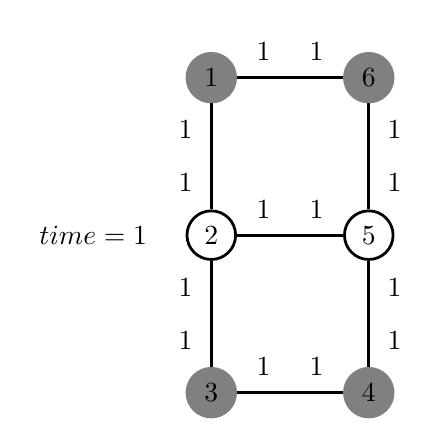
\begin{tikzpicture}[line width=1pt]
      \node at (-1.5,2) {$\text{time} = 1$};
      \tikzstyle{every node}=[circle];
      \node[draw,gray,fill=gray,text=black] (a) at (0,0) {3};
      \node[draw,text=black] (b) at (0,2) {2};
      \node[draw,text=black] (c) at (2,2) {5};
      \node[draw,gray,fill=gray,text=black] (d) at (2,0) {4};
      \node[draw,gray,fill=gray,text=black] (e) at (0,4) {1};
      \node[draw,gray,fill=gray,text=black] (f) at (2,4) {6};
      \draw (a) -- (b) 
      node[near start,left] {1}
      node[near end,left] {1}
      -- (c)
      node[near start,above] {1}
      node[near end,above] {1}
      -- (d)
      node[near start,right] {1}
      node[near end,right] {1}
      -- (a)
      node[near start,above] {1}
      node[near end,above] {1}
      (b) -- (e) 
      node[near start,left] {1}
      node[near end,left] {1}
      -- (f) 
      node[near start,above] {1}
      node[near end,above] {1}
      -- (c)
      node[near start,right] {1}
      node[near end,right] {1};
    \end{tikzpicture}
    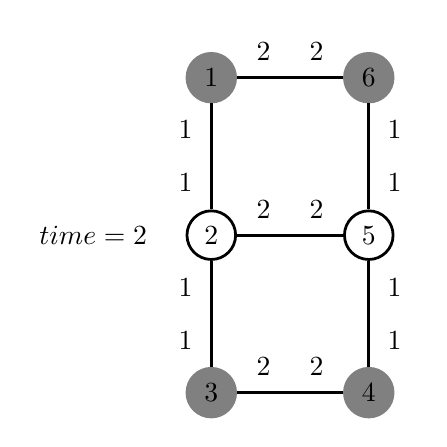
\begin{tikzpicture}[line width=1pt]
      \tikzstyle{every node}=[circle];
      \node at (-1.5,2) {$\text{time} = 2$};
      \node[draw,gray,fill=gray,text=black] (a) at (0,0) {3};
      \node[draw,text=black] (b) at (0,2) {2};
      \node[draw,text=black] (c) at (2,2) {5};
      \node[draw,gray,fill=gray,text=black] (d) at (2,0) {4};
      \node[draw,gray,fill=gray,text=black] (e) at (0,4) {1};
      \node[draw,gray,fill=gray,text=black] (f) at (2,4) {6};
      \draw (a) -- (b) 
      node[near start,left] {1}
      node[near end,left] {1}
      -- (c)
      node[near start,above] {2}
      node[near end,above] {2}
      -- (d)
      node[near start,right] {1}
      node[near end,right] {1}
      -- (a)
      node[near start,above] {2}
      node[near end,above] {2}
      (b) -- (e) 
      node[near start,left] {1}
      node[near end,left] {1}
      -- (f) 
      node[near start,above] {2}
      node[near end,above] {2}
      -- (c)
      node[near start,right] {1}
      node[near end,right] {1};
    \end{tikzpicture}

    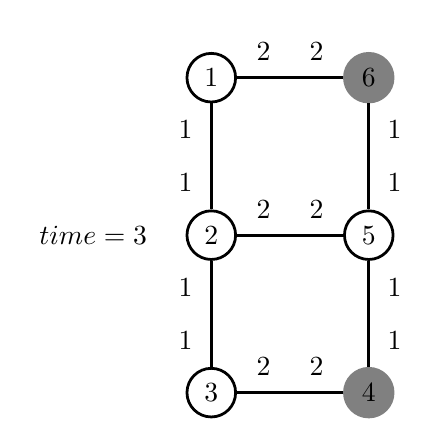
\begin{tikzpicture}[line width=1pt]
      \node at (-1.5,2) {$\text{time} = 3$};
      \tikzstyle{every node}=[circle];
      \node[draw,text=black] (a) at (0,0) {3};
      \node[draw,text=black] (b) at (0,2) {2};
      \node[draw,text=black] (c) at (2,2) {5};
      \node[draw,gray,fill=gray,text=black] (d) at (2,0) {4};
      \node[draw,text=black] (e) at (0,4) {1};
      \node[draw,gray,fill=gray,text=black] (f) at (2,4) {6};
      \draw (a) -- (b) 
      node[near start,left] {1}
      node[near end,left] {1}
      -- (c)
      node[near start,above] {2}
      node[near end,above] {2}
      -- (d)
      node[near start,right] {1}
      node[near end,right] {1}
      -- (a)
      node[near start,above] {2}
      node[near end,above] {2}
      (b) -- (e) 
      node[near start,left] {1}
      node[near end,left] {1}
      -- (f) 
      node[near start,above] {2}
      node[near end,above] {2}
      -- (c)
      node[near start,right] {1}
      node[near end,right] {1};
    \end{tikzpicture}
    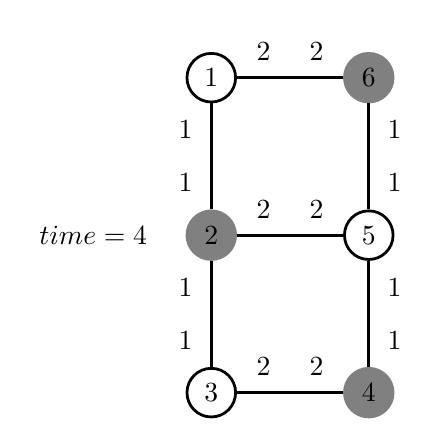
\begin{tikzpicture}[line width=1pt]
      \node at (-1.5,2) {$\text{time} = 4$};
      \tikzstyle{every node}=[circle];
      \node[draw,text=black] (a) at (0,0) {3};
      \node[draw,gray,fill=gray,text=black] (b) at (0,2) {2};
      \node[draw,text=black] (c) at (2,2) {5};
      \node[draw,gray,fill=gray,text=black] (d) at (2,0) {4};
      \node[draw,text=black] (e) at (0,4) {1};
      \node[draw,gray,fill=gray,text=black] (f) at (2,4) {6};
      \draw (a) -- (b) 
      node[near start,left] {1}
      node[near end,left] {1}
      -- (c)
      node[near start,above] {2}
      node[near end,above] {2}
      -- (d)
      node[near start,right] {1}
      node[near end,right] {1}
      -- (a)
      node[near start,above] {2}
      node[near end,above] {2}
      (b) -- (e) 
      node[near start,left] {1}
      node[near end,left] {1}
      -- (f) 
      node[near start,above] {2}
      node[near end,above] {2}
      -- (c)
      node[near start,right] {1}
      node[near end,right] {1};
    \end{tikzpicture}
  \end{center}
  \end{minipage}
  \caption{Example of distributed breakout. The only colors allowed
    are white and gray. The numbers represent the weights that the
    agents give to each of their constraints. We show four steps,
    starting at the top left.}
  \label{fig:dbex}
\end{SCfigure}


The full algorithm can be seen in figure~\ref{fig:dbreakout}. In it we
can see that the agents spend their time either waiting to
$\proc{handle-ok?}$ or $\proc{handle-improve}$ from all their
neighbors. Once an agent gets all the $\proc{handle-ok?}$ invocations
it calculates its new cost and possible improvement and sends a
\proc{handle-improve} to all its neighbors.  Once an agent gets all
the \proc{handle-improve} messages then the agent determines if it is
in a quasi-local-minimum.  If so then it increases the weights of the
constraint violations and sends a \proc{handle-ok?} to its neighbors.

\netlogo{DBgc} Figure~\ref{fig:dbex} shows an example application of
the distributed breakout algorithm. We start out with a random
coloring for all the nodes as seen on the first picture on the left.
Once the agents receive all the \proc{handle-ok?} from their neighbors
they check to see how much they could improve by changing and send the
\proc{handle-improve} messages. In this case, it turns out that for
all agents $\id{my-improve} \leq 0$. Therefore, the agents increase
weights to that shown on the second picture. At this point nodes 1, 2,
4 and 6 have a $\id{my-improve} = 1$ while 2, 5 are at $-3$. We break
ties using the agent number where smaller number wins. As such, agents
1 and 3 are the ones that get to change their color. They do so in the
third picture. They then tell their neighbors their new color by
calling \proc{handle-ok?} on them. At this point agent 2 has a
$\id{my-improve} = 4$ (that is $1 + 1 + 2$) which is higher than
anyone else's so it gets to change its color which moves us to the
last picture.

The performance of distributed breakout is, on average, superior to
\acro{awc} which is in turn superior to \acro{abt}.  However, we
should always remember that distributed breakout is not complete.

\begin{theorem}[Distributed Breakout is \textbf{not} Complete]
\label{th:dbnotc}
  Distributed breakout can get stuck in local minimum. Therefore,
  there are cases where a solution exists and it cannot find it.
\end{theorem}

Distributed breakout will also not be able to identify that a
particular problem lacks a solution. Specifically, the algorithm will
either continue running or get stuck in a local minimum when given a
problem that lacks a solution. As such, breakout cannot be used when
there is any chance that the problem lacks a solution and you want to
determine if the problem has or does not have a solution.

Tests have also shown that the load distribution of distributed
breakout is uneven.  That is, some agents end up handling several
times more messages than other agents. There is likely a correlation
between the number of edges an agent has and the number of messages it
must process. Still, distributed breakout has been shown to, in
practice, find the local optima a very large percentage of the time,
and variations of the basic algorithm perform even better.
Specifically, \td{Multi-DB$^{++}$} has been shown to, in practice,
always find the solution for 3SAT problems \cite{hirayama05a}.


\section{Distributed Constraint Optimization}
\label{sec:dcop}


The \td{distributed constraint optimization} problem is similar to the
constraint satisfaction problem except that the constraints return a
real number instead of a boolean value and the goal is to minimize the
value of these constraint violations. The problem arises when
multiple, perhaps all, solutions are valid but some are preferred to
others. For example, say you are trying to schedule all your classes
or weekly meetings and any schedule where no class overlaps another
one is a valid schedule. However, you might prefer schedules with the
least number of early morning classes.

We formally define a constraint optimization problem as follows:


\begin{definition}[Constraint Optimization Problem (\acro{cop})]
  Given a set of variables $x_1, x_2,\ldots x_n$ with domains $D_1,
  D_2,\ldots D_n$ and a set of constraints $P$ of the form $pk(x_{k1},
  x_{k2},\ldots, x_{kj}) \rightarrow \Re$, find assignments for all
  the variables such that the sum of the constraint values is
  minimized.
\end{definition}

\acro{cop} is an NP-Complete problem. That means that, at worse, all
algorithms will take an exponential time (in the number of variables)
to finish. Even parallel algorithms will, at worst, need exponential
time. However, those are worst case scenarios. In practice we find
some algorithms that do very well on most problems.


\begin{SCfigure}
  \begin{minipage}{1.0\linewidth}
    \begin{codebox}
      \Procname{$\proc{branch-and-bound-cop}()$}
      \li $c* \gets \infty$ \>\>\>\Comment Minimum cost found. Global variable.
      \li $g* \gets \emptyset$ \>\>\>\Comment Best solution found. Global
      variable.
      \li $\proc{branch-and-bound-cop-helper}(1,\emptyset)$
      \li \Return $g^*$
    \end{codebox}
    \begin{codebox}
    \Procname{$\proc{branch-and-bound-cop-helper}(i,g)$}
    \li \If $i = n$ 
    \li \Then \If $P(g) < c^*$ \Comment Cost of violations in $g$ is
    less than current bound.
    \li       \Then $g^* \gets g$
    \li             $c^* \gets P(g)$
              \End
    \li       \Return
        \End              
    \li \For $v \in D_i$ 
    \li \Do $g' \gets g + \{x_i \gets v\}$
    \li     \If $P(g') < c^*$
    \li     \Then \proc{branch-and-bound-cop-helper}$(i+1, g')$
            \End
        \End
  \end{codebox}
  \end{minipage}
  \caption{A centralized branch and bound algorithm for constraint
    optimization. It assumes there are $n$ variables,
    $x_1,\ldots,x_n$, and that $P(g)$ returns the total of any
    constraint violations given partial assignment $g$ and constraints
    $P$.}
  \label{fig:bb-cop}
\end{SCfigure}

The most common approach to solving \acro{cop}s is to use a \td{branch and
  bound} algorithm such as the one shown in figure~\ref{fig:bb-cop}.
Branch and bound algorithms perform a depth first search of the
variable assignments but also maintain a bound, $c^*$, which is the
cost of the best solution found thus far. If a partial variable
assignment already has a cost that is equal or higher than $c^*$ then
we know that there is no need to find values for the rest of the
variables as the cost will only increase. The algorithm is complete so
it will find the best possible solution to the problem, but doing so
might require a lot of time. Since it is based on a depth first search
its memory requirements are linear on the number of
variables. 

The distributed constraint optimization problem distributes the
variables to the agents.

\begin{definition}[Distributed Constraint Optimization Problem (\acro{dcop})]
  Give each agent one of the variables in a \acro{cop}. Agents are
  responsible for finding a value for their variable and can find
  out the values of their neighbors' via communication
\end{definition}

We now look at some algorithms for solving the \acro{dcop} problem.

\subsection{Adopt}

\begin{SCfigure}
  \begin{minipage}{1.0\linewidth}
    \begin{codebox}
      \Procname{$\proc{reset-variables}(d,c)$}
      \li $\id{lower-bound}[d,c] \gets 0$
      \li $t[d,c] \gets 0$
      \li $\id{upper-bound}[d,c] \gets \infty$
      \li$\id{context}[d,c] \gets  \{\}$
    \end{codebox}
    \begin{codebox}
      \Procname{$\proc{initialize}()$}
      \li $\id{threshold} \gets 0$
      \li $\id{received-terminate} \gets \const{false}$
      \li $\id{current-context} \gets \{\}$
      \li $\forall_{d \in D_i, c \in \id{children}} \; \proc{reset-variables}(d,c)$
      \li $x_i \gets d \in D_i$ which minimizes: my cost plus $\sum_{c \in
        \id{children}} \id{lower-bound}[d,c]$
      \li $\proc{backtrack}()$
    \end{codebox}
    \begin{codebox}
      \Procname{$\proc{handle-threshold}(t,\id{context})$}
      \li \If \id{context} is compatible with \id{current-context}
      \li   \Then $\id{threshold} \gets t$
      \li         $\proc{maintain-threshold-invariant}()$
      \li         $\proc{backtrack}()$
          \End
    \end{codebox}
    \begin{codebox}
      \Procname{$\proc{handle-terminate}(\id{context})$}
      \li $\id{received-terminate} \gets \const{true}$
      \li $\id{current-context} \gets \id{context}$
      \li $\proc{backtrack}()$
    \end{codebox}
    \begin{codebox}
      \Procname{$\proc{handle-value}(j,x_j)$}
      \li \If $\neg \id{received-terminate}$
      \li \Then $\id{current-context}[j] \gets x_j$
      \li \For $d \in D_i, c \in \id{children}$ such that
      $\id{context}[d,c]$ is 
      \zi \>\>\>\>\>\>incompatible with \id{current-context}
      \li \Do  $\proc{reset-variables}(d,c)$
          \End
      \li  $\proc{maintain-threshold-invariant}()$
      \li  $\proc{backtrack}()$
          \End
    \end{codebox}
    \begin{codebox}
      \Procname{$\proc{handle-cost}(k,\id{context}, \id{lb},\id{ub})$}
      \li $d \gets \id{context}[i]$
      \li \kw{delete} $\id{context}[i]$
      \li \If $\neg \id{received-terminate}$
      \li \Then \For $(j,x_j) \in \id{context}$ and $j$ is not my
      neighbor
      \li       \Do $\id{current-context}[j] \gets x_j$
                \End
      \li       \For $d' \in D_i, c \in \id{children}$ such that
      $\id{context}[d,c]$ is 
      \zi       \>\>\>\>\>\>incompatible with \id{current-context}
      \li       \Do  $\proc{reset-variables}(d',c)$
          \End
      \li \If $\id{context}$ compatible with \id{current-context}
      \li \Then $\id{lower-bound}[d,k] \gets lb$
      \li       $\id{upper-bound}[d,k] \gets ub$
      \li       $\id{context}[d,k] \gets \id{context}$
      \li       $\proc{maintain-child-threshold-invariant}()$
      \li       $\proc{maintain-threshold-invariant}()$
          \End
      \li $\proc{backtrack}()$
    \end{codebox}
  \end{minipage}
  \caption{The Adopt algorithm. Before the algorithm is even
    called the agents must form a depth first search tree. Each agent
    has a \id{parent} variable which points to its parent. The root's
    parent is set as null.}
  \label{fig:adopt}
\end{SCfigure}

The \td{Adopt} algorithm \cite{modi04a} is a recent addition to the
family of \acro{dcop} algorithms. It is roughly a depth-first search
on the set of possible value assignments, but with a lot of
improvements on the basic search strategy. Namely, each agent in the
depth-first tree keeps a lower and upper bound on the cost for the
sub-problem below him (given assignments from above) and on the
sub-problems for each one of his children. It then tells the children
to look for a solution but ignore any partial solution whose cost is
above the lower bound because it already knows that it can get that
lower cost.


\begin{SCfigure}
  \begin{minipage}{1.0\linewidth}
    \begin{codebox}
      \Procname{$\proc{backtrack}()$}
      \li \If $\id{threshold} = \min_{d \in D_i} \func{cost}(d) + \sum_{c
        \in \id{children}} \id{upper-bound}[d,c]$
      \li \Then $x_i \gets \arg \min_{d \in D_i} \func{cost}(d) + \sum_{c
        \in \id{children}} \id{upper-bound}[d,c]$
      \li \ElseIf $\id{threshold} < \func{cost}(x_i) + \sum_{c \in
        \id{children}} \id{lower-bound}[x_i,c]$
      \li \Then $x_i \gets \arg \min_{d \in D_i} \func{cost}(d) + \sum_{c \in
        \id{children}} \id{lower-bound}[d,c]$
          \End
      \li $\forall_{k \in \id{neighbors} \wedge k \text{ has lower
          priority}} k.\proc{handle-value}(i,x_i)$
      \li $\proc{maintain-allocation-invariant}()$
      \li \If $\id{threshold} = \min_{d \in D_i} \func{cost}(d) + \sum_{c
        \in \id{children}} \id{upper-bound}[d,c]$ and
      \zi \>\>\>      (\id{received-terminate} or I am root)
      \li \Then $\id{current-context}[i] \gets x_i$
      \li       $\forall_{c \in \id{children}} c.\proc{handle-terminate}(\id{current-context})$
      \li       $\kw{exit}$
          \End
      \li $\id{parent}.\proc{handle-cost}(\id{current-context},$
      \zi \>\>$\min_{d \in D_i} \func{cost}(d) + \sum_{c \in
        \id{children}} \id{lower-bound}[d,c],$
      \zi \>\>$\min_{d \in D_i} \func{cost}(d) + \sum_{c \in \id{children}}
      \id{upper-bound}[d,c])$
    \end{codebox}
    \begin{codebox}
      \Procname{$\proc{maintain-threshold-invariant}()$}
      \li \If $\id{threshold} < \min_{d \in D_i} \func{cost}(d) + \sum_{c \in
        \id{children}} \id{lower-bound}[d,c]$
      \li \Then $\id{threshold} \gets \min_{d \in D_i} \func{cost}(d) + \sum_{c \in \id{children}} \id{lower-bound}[d,c]$
          \End
      \li \If $\id{threshold} > \min_{d \in D_i} \func{cost}(d) + \sum_{c
        \in \id{children}} \id{upper-bound}[d,c]$
      \li \Then $\id{threshold} \gets \min_{d \in D_i} \func{cost}(d) + \sum_{c
        \in \id{children}} \id{upper-bound}[d,c]$
          \End
    \end{codebox}
    \begin{codebox}
      \Procname{$\proc{maintain-allocation-invariant}()$}
      \li \While $\id{threshold} > \func{cost}(x_i) + \sum_{c \in
        \id{children}} t[x_i,c]$
      \li \Do $\id{chosen} \gets c' \in \id{children} \text{ such that
        } \id{upper-bound}[x_i,c'] > t[x_i,c']$
      \li     $t[x_i,\id{chosen}] \gets t[x_i,\id{chosen}] + 1$
          \End
      \li \While $\id{threshold} < \func{cost}(x_i) + \sum_{c \in
        \id{children}} t[x_i,c]$
      \li \Do $\id{chosen} \gets c' \in \id{children} \text{ such that
        } \id{lower-bound}[x_i,c'] < t[x_i,c']$
      \li     $t[x_i,\id{chosen}] \gets t[x_i,\id{chosen}] - 1$
          \End
      \li $\forall_{c \in \id{children}}
      c.\proc{handle-threshold}(t[x_i,\id{chosen}], \id{current-context})$
    \end{codebox}
    \begin{codebox}
      \Procname{$\proc{maintain-child-threshold-invariant}()$}
      \li \For $d \in D_i, c \in \id{children}$
      \li \Do \If $\id{lower-bound}[d,c] > t[d,c]$
      \li     \Then $t[d,c] \gets \id{lower-bound}[d,c]$
              \End
          \End
      \li \For $d \in D_i, c \in \id{children}$
      \li \Do \If $\id{upper-bound}[d,c] < t[d,c]$
      \li     \Then $t[d,c] \gets \id{upper-bound}[d,c]$
              \End
          \End
    \end{codebox}
  \end{minipage}
  \caption{The Adopt algorithm, continued.}
  \label{fig:adopt2}
\end{SCfigure}
%There are three basic types of messages in Adopt.

%\begin{itemize}
%\item $\mathbf{threshold}$ tell children how much cost they can
%  incur, ignore anything that costs more than that.
%\item $\mathbf{value}$ tell descendants what value agent sets itself
%  to.
%\item $\mathbf{cost}$ tell parent lower and upper bounds of cost
%  given the current value assignments of ancestors.
%\end{itemize}

The general idea in Adopt is that each node in the tree calculates
upper and lower bounds on the cost for all the constraints that
involve all the nodes in the subtree rooted at that node, given an
assignment for the nodes on the path to the root. Each node changes to
the value (color) whose lower bound is smallest at each time and then
asks its children to calculate new bounds given the new value. Upon
receiving this message each node again changes its value to the one
with the lowest lower bound and the process is repeated.
Figures~\ref{fig:adopt} and~\ref{fig:adopt2} show the full algorithm.

\begin{SCtable}
  \begin{minipage}{1.0\linewidth}
  \begin{center}
    \begin{tabular}[c]{ccc} \toprule
      $d_i$ & $d_j$ & $p(d_i,d_j)$ \\ \midrule
      0 & 0 & 1 \\
      0 & 1 & 2 \\
      1 & 0 & 2 \\
      1 & 1 & 0 \\ \bottomrule
    \end{tabular}
  \end{center}
  \end{minipage}
  \caption{Cost function for Adopt example in figure~\ref{fig:adoptex}.}
  \label{tab:adoptcost}
\end{SCtable}

\begin{SCfigure}
  \begin{minipage}{1.0\linewidth}
  \begin{center}
    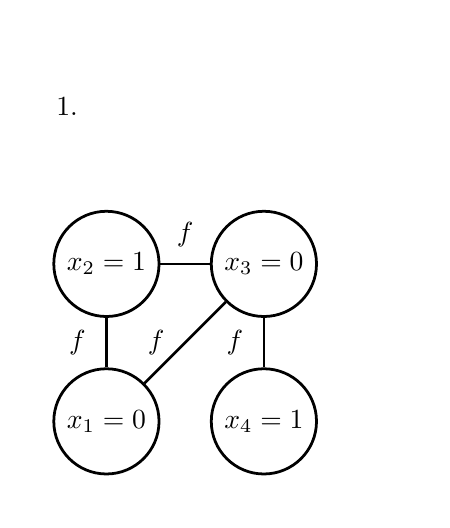
\begin{tikzpicture}[line width=1pt]
      \useasboundingbox (-1,-1) rectangle (4,5);
      \node at (-.5,4) {$1.$};
      \node[draw,circle] (x1) at (0,0) {$x_1 = 0$};
      \node[draw,circle] (x2) at (0,2) {$x_2 = 1$};
      \node[draw,circle] (x3) at (2,2) {$x_3 = 0$};
      \node[draw,circle] (x4) at (2,0) {$x_4 = 1$};
      \draw (x1) -- node[left] {$f$} (x2);
      \draw (x1) -- node[left] {$f$} (x3);
      \draw (x2) -- node[above] {$f$} (x3);
      \draw (x3) -- node[left] {$f$} (x4);
    \end{tikzpicture}
    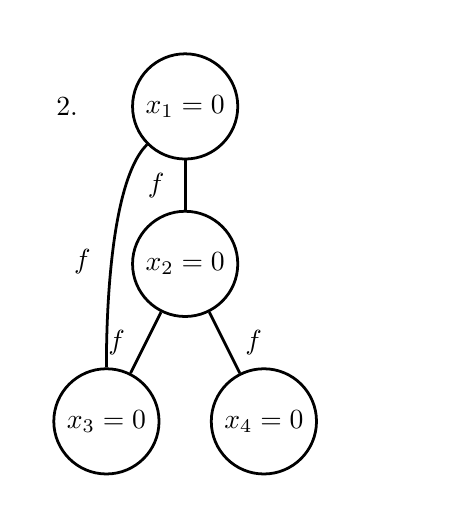
\begin{tikzpicture}[line width=1pt]
      \useasboundingbox (-1,-1) rectangle (4,5);
      \node at (-.5,4) {$2.$};
      \node[draw,circle] (x1) at (1,4) {$x_1 = 0$};
      \node[draw,circle] (x2) at (1,2) {$x_2 = 0$};
      \node[draw,circle] (x3) at (0,0) {$x_3 = 0$};
      \node[draw,circle] (x4) at (2,0) {$x_4 = 0$};
      \draw (x1) -- node[left] {$f$} (x2);
      \draw (x1) .. controls +(-1,-1) and +(0,1) .. node[left] {$f$} (x3);
      \draw (x2) -- node[left] {$f$} (x3);
      \draw (x2) -- node[right] {$f$} (x4);
    \end{tikzpicture}
    \begin{tikzpicture}[line width=1pt]
      \useasboundingbox (-1,-1) rectangle (4,5);
      \node at (-.5,4) {$3.$};
      \node[draw,circle] (x1) at (1,4) {$x_1 = 0$};
      \node[draw,circle] (x2) at (1,2) {$x_2 = 0$};
      \node[draw,circle] (x3) at (0,0) {$x_3 = 0$};
      \node[draw,circle] (x4) at (2,0) {$x_4 = 0$};
      \draw (x1) -- (x2);
      \draw (x1) .. controls +(-1,-1) and +(0,1) .. (x3);
      \draw (x2) -- (x3);
      \draw (x2) -- (x4);
      \draw[black,-angle 90] (x1) .. controls +(-2,-2)
      .. node[left] {\begin{tabular}{c}
          $\mathbf{value}$ \\
          $x_1 = 0$
        \end{tabular}} (x3);
      \draw[black,-angle 90] (x1) .. controls +(1,-1)
      .. node[right] {\begin{tabular}{c}
          $\mathbf{value}$ \\
          $x_1 = 0$
        \end{tabular}} (x2);
      \draw[black,-angle 90] (x2) .. controls +(0,-1)
      .. (x3);
      \draw[black,-angle 90] (x2) .. controls +(1,-1)
      .. node[right] {\begin{tabular}{c}
          $\mathbf{value}$ \\
          $x_2 = 0$
        \end{tabular}} (x4);
    \end{tikzpicture}
    \begin{tikzpicture}[line width=1pt]
      \useasboundingbox (-1,-1) rectangle (4,5);
      \node at (-.5,4) {$4.$};
      \node[draw,circle] (x1) at (1,4) {$x_1 = 0$};
      \node[draw,circle] (x2) at (1,2) {$x_2 = 0$};
      \node[draw,circle] (x3) at (0,0) {$x_3 = 0$};
      \node[draw,circle] (x4) at (2,0) {$x_4 = 0$};
      \draw (x1) -- (x2);
      \draw (x1) .. controls +(-1,-1) and +(0,1) .. (x3);
      \draw (x2) -- (x3);
      \draw (x2) -- (x4);
      \draw[black,-angle 90] (x2) .. controls +(1,1)
      .. node[right] {\begin{tabular}{c}
          $\mathbf{cost}$ \\
          1,$\infty$ \\
          $x_1 = 0$
        \end{tabular}} (x1);
      \draw[black,-angle 90] (x3) .. controls +(-1,1) and +(-1,0)
      .. node[left] {\begin{tabular}{c}
          $\mathbf{cost}$ \\
          2,2 \\
          $x_1 = 0$\\
          $x_2=0$
        \end{tabular}} (x2);
      \draw[black,-angle 90] (x4) .. controls +(1,1) 
      .. node[right] {\begin{tabular}{c}
          $\mathbf{cost}$ \\
          1,1 \\
          $x_2 = 0$
        \end{tabular}} (x2);
    \end{tikzpicture}

    \begin{tikzpicture}[line width=1pt]
      \useasboundingbox (-1,-1) rectangle (4,5);
      \node at (-.5,4) {$5.$};
      \node[draw,circle] (x1) at (1,4) {$x_1 = 1$};
      \node[draw,circle] (x2) at (1,2) {$x_2 = 0$};
      \node[draw,circle] (x3) at (0,0) {$x_3 = 0$};
      \node[draw,circle] (x4) at (2,0) {$x_4 = 0$};
      \draw (x1) -- (x2);
      \draw (x1) .. controls +(-1,-1) and +(0,1) .. (x3);
      \draw (x2) -- (x3);
      \draw (x2) -- (x4);
      \draw[black,-angle 90] (x1) .. controls +(-2,-2)
      .. node[left] {\begin{tabular}{c}
          $\mathbf{value}$ \\
          $x_1 = 1$
        \end{tabular}} (x3);
      \draw[black,-angle 90] (x1) .. controls +(1,-1)
      .. node[right] {\begin{tabular}{c}
          $\mathbf{value}$ \\
          $x_1 = 1$
        \end{tabular}} (x2);
    \end{tikzpicture}
    \begin{tikzpicture}[line width=1pt]
      \useasboundingbox (-1,-1) rectangle (4,5);
      \node at (-.5,4) {$6.$};
      \node[draw,circle] (x1) at (1,4) {$x_1 = 1$};
      \node[draw,circle] (x2) at (1,2) {$x_2 = 1$};
      \node[draw,circle] (x3) at (0,0) {$x_3 = 1$};
      \node[draw,circle] (x4) at (2,0) {$x_4 = 0$};
      \draw (x1) -- (x2);
      \draw (x1) .. controls +(-1,-1) and +(0,1) .. (x3);
      \draw (x2) -- (x3);
      \draw (x2) -- (x4);
      \draw[black,-angle 90] (x2) .. controls +(1,1)
      .. node[right] {\begin{tabular}{c}
          $\mathbf{cost}$ \\
          0,$\infty$ \\
          $x_1 = 1$
        \end{tabular}} (x1);
      \draw[black,-angle 90] (x3) .. controls +(-1,1) and +(-1,0)
      .. node[left] {\begin{tabular}{c}
          $\mathbf{cost}$ \\
          2,2 \\
          $x_1=1$\\
          $x_2=0$
        \end{tabular}} (x2);
      \draw[black,-angle 90] (x2) .. controls +(0,-1)
      .. (x3);
      \draw[black,-angle 90] (x2) .. controls +(1,-1)
      .. node[right] {\begin{tabular}{c}
          $\mathbf{value}$ \\
          $x_2 = 1$
        \end{tabular}} (x4);
    \end{tikzpicture}

    \begin{tikzpicture}[line width=1pt]
      \useasboundingbox (-1,-1) rectangle (4,5);
      \node at (-.5,4) {$7.$};
      \node[draw,circle] (x1) at (1,4) {$x_1 = 1$};
      \node[draw,circle] (x2) at (1,2) {$x_2 = 1$};
      \node[draw,circle] (x3) at (0,0) {$x_3 = 1$};
      \node[draw,circle] (x4) at (2,0) {$x_4 = 1$};
      \draw (x1) -- (x2);
      \draw (x1) .. controls +(-1,-1) and +(0,1) .. (x3);
      \draw (x2) -- (x3);
      \draw (x2) -- (x4);
      \draw[black,-angle 90] (x2) .. controls +(1,1)
      .. node[right] {\begin{tabular}{c}
          $\mathbf{cost}$ \\
          0,3 \\
          $x_1 = 1$
        \end{tabular}} (x1);
      \draw[black,-angle 90] (x3) .. controls +(-1,1) and +(-1,0)
      .. node[left] {\begin{tabular}{c}
          $\mathbf{cost}$ \\
          0,0 \\
          $x_1=1$\\
          $x_2=1$
        \end{tabular}} (x2);
      \draw[black,-angle 90] (x4) .. controls +(1,1) 
      .. node[right] {\begin{tabular}{c}
          $\mathbf{cost}$ \\
          0,0 \\
          $x_2 = 1$
        \end{tabular}} (x2);
    \end{tikzpicture}
    \begin{tikzpicture}[line width=1pt]
      \useasboundingbox (-1,-1) rectangle (4,5);
      \node at (-.5,4) {$8.$};
      \node[draw,circle] (x1) at (1,4) {$x_1 = 1$};
      \node[draw,circle] (x2) at (1,2) {$x_2 = 1$};
      \node[draw,circle] (x3) at (0,0) {$x_3 = 1$};
      \node[draw,circle] (x4) at (2,0) {$x_4 = 1$};
      \draw (x1) -- (x2);
      \draw (x1) .. controls +(-1,-1) and +(0,1) .. (x3);
      \draw (x2) -- (x3);
      \draw (x2) -- (x4);
      \draw[black,-angle 90] (x2) .. controls +(1,1)
      .. node[right] {\begin{tabular}{c}
          $\mathbf{cost}$ \\
          0,0 \\
          $x_1 = 1$
        \end{tabular}} (x1);
    \end{tikzpicture}
  \end{center}
  \end{minipage}
  \caption{Adopt example. Start at the top left and read left to
    right. The domain for all nodes is the set $\{0,1\}$.}
  \label{fig:adoptex}
\end{SCfigure}

The basic workings of Adopt are best shown via an example.
Table~\ref{tab:adoptcost} shows the cost function we will be using in
our example.  Figure~\ref{fig:adoptex} shows a trace of an application
of Adopt to a simple problem. As you can see, all the constraints are
binary, as Adopt can only handle binary constraints. All the agents
keep track of the upper and lower bounds sent by their children along
with the associated context.  They use these bounds to calculate
bounds on their own costs.  Initially, all lower bounds are set to 0
and all upper bounds to infinity.

The first diagram is the constraints graph itself. The first thing we
must do before even starting Adopt is to form a depth-first search
graph. That is, a graph such that all constraints emanating from a
node go to either one of its descendants---the tree below it---or one
of its ancestors---agents on the path from the node to the root. There
exists several algorithms for finding such a tree and generally
multiple trees can be formed from one constraints graph. The second
diagram shows a possible depth-first search tree for our example.

The third diagram shows the first step in the algorithm. All the nodes
invoke \proc{handle-value} on all the descendants with whom they share
a constraint. That is why $x_1$ sends a message to $x_3$ but not
$x_4$. These \proc{handle-value} are similar to the \proc{handle-ok?}
functions we saw before. They simply inform the other agents of the
new value, in this case the original values.

\netlogo{ADOPTgc} The agents use these values to calculate both upper
and lower bounds on their cost and report these back up to their
parents, as shown in the fourth diagram. For example, $x_3$ calculated
that, given that $x_1=0$ and $x_2=0$ if it set itself to 0 the cost
would be 2 and if set itself to 1 the cost would be 4, remember that
we are using the cost function from Table~\ref{tab:adoptcost}, thus
it stays at 0 and sends a \proc{handle-cost} to its parent saying that
its lower and upper bounds, given $x_1=0$ and $x_2=0$, are 2. This
message means that the cost of the constraints for the subtree rooted
at $x_3$ (since $x_3$ is a leaf this then means just all the
constraints in which $x_3$ is involved) given $x_1=0$ and $x_2=0$, are
no lower or no higher than 2.  $x_3$ can set both its upper and lower
bounds because it has values for all its constraints.  On the other
hand, $x_2$ sends an upper bound of $\infty$ because it does not know
the upper bounds of its children, so it does not know how much those
costs could add up to.

In the fifth diagram the agents calculate new best values and so $x_1$
sends \proc{handle-value} messages. In the sixth diagram $x_2$
receives the cost messages from before and sets himself to 1 because
the value 1 has a lower lower bound (because all lower bounds are
initially set to 0). $x_2$ then sends the appropriate
\proc{handle-value} messages.

In the seventh diagram both $x_3$ and $x_4$ calculate that both their
upper and lower bounds are 0 given that $x_1=0$ and $x_2=0$ and send
this message up to $x_2$. In the eighth diagram $x_2$ uses this
message to calculate its new bounds, also 0 and 0, and sends these up
to the root. Upon receiving this message the root knows it can stop
the algorithm because it has identical upper and lower bounds. We note
that the Adopt algorithm is actually a bit more complicated than this
example shows as we ignored any \proc{handle-threshold} invocations.

Test results on Adopt show that there is a very wide discrepancy in
the number of messages each agent must handle and, therefore, the
individual workload.  Namely, agents at the leafs of the tree end up
doing all of the work while the root sits idle. This gets worse as the
tree becomes thinner (like a line). Since the tree must be a
depth-first search graph, this means that problems with a lot of
constraints will be doubly bad because they will need a thinner tree
and the extra constraints means more work for the agents.

Also, it must be noted that if each agent handles each message as it
comes (and calls the \proc{backtrack} routine) then Adopt will never
finish. For Adopt to work the agents need to accumulate a number of
\proc{handle-value} and \proc{handle-cost} invocations before running
their \proc{backtrack} procedure.

\subsection{OptAPO}
\newcommand{\optapo}{opt\acro{apo}}

A different approach to solving the distributed constraint
optimization problem was taken by the Optimizing Asynchronous Partial
Overlay (\tdi{\optapo}{optAPO}) algorithm \cite{mailler04b}, which is the
cousin of the \tdi{\acro{apo}}{APO} algorithm \cite{mailler04a} for
distributed constraint satisfaction.

Both of these algorithms use the same basic idea. The agents start out
doing individual hill-climbing, that is, each one changes its color so
as to minimize constraints violations with its neighbors.  When an
agent realizes that it cannot find a value with no violations it tries
to find a coloring for a (growing) set of agents which includes
itself.  More specifically, each agent maintains a variable called its
\id{good-list} which initially contains only the agent. As the agent
finds conflicts with other agents that it cannot resolve it adds these
agents to its \id{good-list}. Then, the conflict is resolved by
electing one of the agents in the conflict to be the \emph{mediator}
of the conflict. The mediator agent then finds a coloring for all the
agents in its \id{good-list} and which minimizes violations with
agents outside the \id{good-list} using any centralized algorithm,
such as the branch and bound algorithm from figure~\ref{fig:bb-cop}.
The agent then informs the other agents of their new color. The agents
change to their new color as instructed by the mediator.


\begin{SCfigure}
  \begin{minipage}{1.0\linewidth}
  \begin{center}
    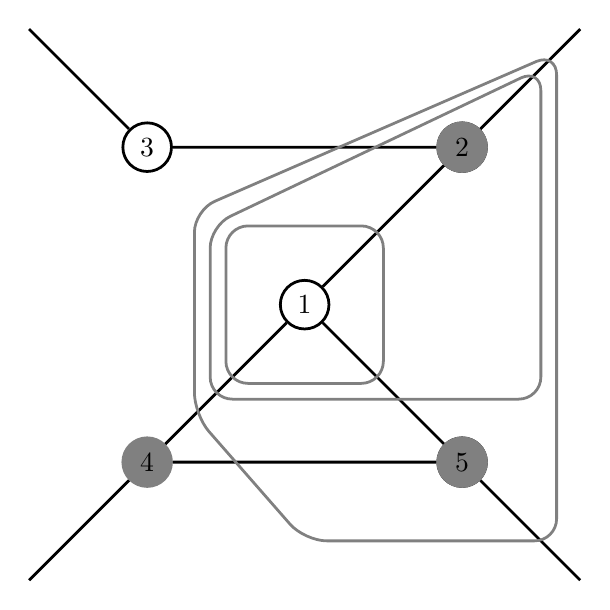
\begin{tikzpicture}[line width=1pt]
      \tikzstyle{every node}=[circle];
      \node[draw,text=black] (a) at (0,0) {1};
      \node[draw,fill=white,text=black] (b) at (2,2) {2};
      \node[draw,fill=white,text=black] (c) at (-2,2) {3};
      \node[draw,gray,fill=gray,text=black] (d) at (-2,-2) {4};
      \node[draw,fill=white,text=black] (e) at (2,-2) {5};
      \draw (a) -- (b) -- (c)
      (a) -- (d) -- (e)
      (a) -- (e)
      (b) -- (3.5,3.5)
      (c) -- (-3.5,3.5)
      (d) -- (-3.5,-3.5)
      (e) -- (3.5,-3.5);

      \draw[rounded corners=8pt,gray]
      (-1,-1) -- (1,-1) -- (1,1) -- (-1,1) -- cycle;


      \draw[rounded corners=8pt,gray]
      (-1.2,-1.2) -- (3,-1.2) -- (3,3) -- (-1.2,1) -- cycle;

      \node[draw,gray,fill=gray,text=black] (b) at (2,2) {2};

      \draw[rounded corners=8pt,gray]
      (-1.4,-1.4) -- (0,-3) -- (3.2,-3) -- (3.2,3.2) -- (-1.4,1.2) -- cycle;
      
      \node[draw,gray,fill=gray,text=black] (e) at (2,-2) {5};
      
    \end{tikzpicture}
  \end{center}
  \end{minipage}
  \caption{Trace of \acro{apo} algorithm showing the growing size of
    node 1's \id{good-list}. Initially only 1 is in the
    \id{good-list}, then 2 joins, finally 5 joins.}
  \label{fig:apo}
\end{SCfigure}
%\netlogo{APOgc}
Figure~\ref{fig:apo} gives an idea of how \acro{apo}
works.  Initially, node 1 has only itself in its \id{good-list}. If it
finds that it cannot resolve a conflict with agent 2 then they enter
into a negotiation phase to elect a mediator. In this case 1 becomes
the mediator and then finds colors for both 1 and 2. Later on another
conflict between 1 and 3 might arise which would lead to 1 becoming
mediator for 1,2,3. Notice that if we give \optapo{} a graph coloring
problem that has no solution, that is, there is always at least one
conflict then it will eventually end up performing a complete depth
first search of the complete problem in one node. This will be
extremely time consuming.

In practice, \acro{apo} and \optapo{} can be very fast, but their
theoretical worst-case bound is still exponential.

\begin{theorem}[\acro{apo} worst case is centralized search]
  \label{th:apowc}
  In the worst case \acro{apo} (\optapo) will make one
  agent do a completely centralized search of the complete problem
  space.
\end{theorem}

\optapo{} requires fewer number of synchronous cycles (that is, steps)
than Adopt but performs a lot more computations as measured by number
of constraints checks \cite{davin05a}. That is, \optapo{} centralizes
the problem much more than Adopt.  When an agent becomes a mediator it
centrally solves a large part of the problem and tells the other
agents what to do. As such, that one agent ends up doing a lot of work
while everyone else does nothing (generally there can be more than one
mediator, each mediating over non-overlapping sets of agents, but this
is rare). In this way \optapo{} can finish in a much smaller number of
steps simply because some of those steps take a long time.

In general we find that Adopt is better when agent to agent
communications are fast and \optapo is better when communications are
slow in comparison to the agent's processing speed. Both of them have
exponential worst-case running times but perform reasonable well for
small problems.

% \section{Recent Advances}
% \label{sec:recent-advances}

% A new algorithm for DCOP based on dynamic programming is presented in
% \cite{petcu05a}. This algorithm is then improved by the ODPOP
% algorithm presented in \cite{petcu06a}.

\begin{exercises}

\item In both \acro{abt} and \acro{awc} the load distribution among
  the agents is very uneven, as demonstrated in our NetLogo
  implementations. Can you come up with an equation that predicts how
  many messages, proportionally, each agent receives given the initial
  problem structure and priorities?

\item The Sodoku puzzle is an instance of a constraint satisfaction
  problem. We can view it as a distributed constraint satisfaction
  problem by simply assuming that each empty square on the board
  corresponds to an agent. \netlogo{DBsodoku}Implement any one of the
  distributed constraint satisfaction algorithms in this chapter to
  solve Sodoku puzzles.

\item Provide an example which proves Theorem~\ref{th:dbnotc}.

\item Provide an example which proves Theorem~\ref{th:apowc}.


\item All these algorithms assume a static constraint
  graph. Unfortunately, many real world applications are dynamic and
  can best be represented by a series of constraint satisfaction
  problems each of which is a little bit different from the previous
  one. In these applications it seems wasteful to re-start the
  algorithm from the beginning when the new problem is only slightly
  different from the old one.

  Implement one of the constraint satisfactions algorithms for graph
  coloring and run tests to determine how it behaves as the graph
  changes. For example, 
  \begin{enumerate}
  \item Start with a randomly generated graph and an initial coloring.
  \item Run the algorithm starting with he current coloring.
  \item Change the graph by adding or deleting a random node.
  \item Goto step 2.
  \end{enumerate}
  Does the algorithm take the same time in the first step as in all
  the other steps? What type of changes to the graph make the most
  difference in the run time?

\end{exercises}

%%% Local Variables: 
%%% mode: latex
%%% TeX-master: "~/wp/mas/mas"
%%% TeX-command-default: "PDFlatex"
%%% End:
